\documentclass[10pt]{article}
\usepackage{graphicx} % Required for inserting images

\title{Receta de pizza}
\author{López Castro Sofía}
\date{Septiembre 2026}

\begin{document}

\maketitle

\begin{figure}[h]
    \centering
    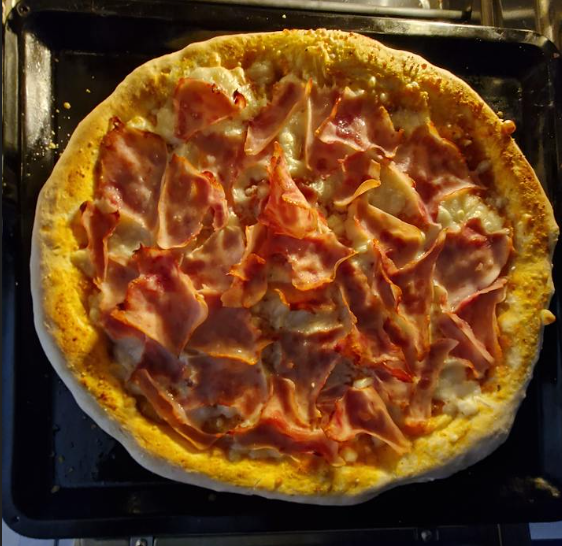
\includegraphics[width=0.6\linewidth]{image.png}
    \caption{Pizza hecha a mano}
    \label{fig:mesh1}
\end{figure}

\section{Ingredientes}

 Para la \textit{masa}:
\begin{itemize}
    \item 400 gr de harina
    \item 11gr de levadura (un sobre)
    \item 1 cucharada de sal
    \item 200ml de agua tibia
    \item 4 cucharadas de aceite (preferentemente de oliva)
\end{itemize}
Para los \textit{aditivos}:
\begin{itemize}
    \item Queso mozzarella 
    \item 6-7 rebanadas de jamón
    \item Sasonador de pizza
\end{itemize}
Para la \textit{salsa}:
\begin{itemize}
    \item 4 tomates
    \item 1 ajo
    \item Óregano seco
\end{itemize} 

\section{Preparación}

\begin{enumerate}
    \item Mezcla el agua, el aceite y la sal en un bowl.
    \item Una vez todo mezclado, calienta el agua hasta que este tibia, una vez tibia agrega la levadura y revuelve.
    \item Deja reposar la mezcla de 5-8 minutos (hasta que se vea que la levadura haya fermentado).
    \item Una vez que la mezcla este fermentada pon la harina en una superficie limpia y haz un volcán.
    \item En medio del volcán agrega la mezcla fermentada y empieza a amasar hasta que la masa no se te pegue en las manos y al momento de estirarla no se rompa tanto. \textbf{Deja reposar una hora o hasta que la masa duplique el tamaño.}
    \item Mientras la masa fermenta, agarra los tomates y cortalos tantito en forma de cruz, después ponlos en una olla con agua a hervir por 10 minutos.
    \item Una vez hervidos les quitas la cáscara y los pones en la licuadora junto con el ajo, un poco de óregano y un chorro pequeño de agua.
    \item Ya mezclados pasa la salsa a una olla a fuego bajo y revuelve hasta que cambie por un color más óscuro.
    \item \textbf{Una vez fermentada la masa} esparsela en una charola y trata de crear un circulo y a la vez delimitar las orillas.
    \item Ya hecho el circulo agrega la salsa, despues el queso, seguido de eso agrega el jamón cortado en trozos o como prefieras, y por último pon sasonador para pizza.
    \item Mete la pizza al horno y déjala de 20-25 minutos.
    \item \textbf{\textit{Y listooooo, ¡Disfruta!}}
    
\end{enumerate}

\end{document}
